% Informe final — Proyecto 2 (CC3084 Data Science, UVG). Compilar con XeLaTeX:
%   xelatex informe_final && bibtex informe_final && xelatex informe_final && xelatex informe_final
% Cifras del EDA de imágenes: python tools/gen_tablas_eda.py  (genera generated/*.tex)
\documentclass[11pt,a4paper]{article}
\usepackage{fontspec}
\usepackage{polyglossia}
\setmainlanguage{spanish}
\usepackage[margin=2.5cm]{geometry}
\usepackage{graphicx,booktabs,float,caption,xcolor,enumitem,array}
\usepackage[most]{tcolorbox}
\usepackage[authoryear,round]{natbib}
\usepackage[hidelinks]{hyperref}
\setlength{\parskip}{4pt}
\captionsetup{font=small,labelfont=bf}
\graphicspath{{figs/}}
% GENERADO por informe/tools/gen_tablas_eda.py: no editar a mano
\newcommand{\tablaChecks}{\begin{tabular}{lrr}
\toprule
Comprobaci\'on & Estudios & \% \\
\midrule
Matriz distinta de $512\times512$ & 3 & 0.15 \\
RescaleIntercept $\notin\{-1024,0\}$ (p.\,ej. $-8192$/$-10240$) & 144 & 7.13 \\
RescaleSlope $\neq 1$ & 141 & 6.98 \\
Dimensiones de matriz variables dentro del estudio & 0 & 0.00 \\
Slope/intercept variables dentro del estudio & 0 & 0.00 \\
SliceThickness variable dentro del estudio & 0 & 0.00 \\
BitsStored fuera de $\{12,16\}$ & 0 & 0.00 \\
PhotometricInterpretation $\neq$ MONOCHROME2 & 0 & 0.00 \\
At\'ipico (IQR$\times$1.5) en n.$^\circ$ de cortes & 27 & 1.34 \\
At\'ipico (IQR$\times$1.5) en SliceThickness & 0 & 0.00 \\
At\'ipico (IQR$\times$1.5) en PixelSpacing & 111 & 5.50 \\
At\'ipico (IQR$\times$1.5) en espaciado $z$ & 2 & 0.10 \\
\bottomrule
\end{tabular}
}
\newcommand{\tablaDesc}{\begin{tabular}{lrrrrr}
\toprule
Variable & Media & D.\,E. & M\'in. & Mediana & M\'ax. \\
\midrule
Cortes por estudio & 352.452 & 132.010 & 69.000 & 314.000 & 1082.000 \\
SliceThickness (mm) & 0.731 & 0.185 & 0.488 & 0.625 & 1.000 \\
PixelSpacing (mm) & 0.328 & 0.078 & 0.190 & 0.312 & 0.713 \\
Espaciado $z$ medido (mm) & 0.626 & 0.204 & 0.312 & 0.625 & 2.626 \\
\bottomrule
\end{tabular}
}

% GENERADO: no editar a mano
\newcommand{\cifNEstudios}{2019}
\newcommand{\cifFuente}{auditoría del pipeline (artifacts/v2/results/dicom\_metadata.csv.gz)}
\newcommand{\cifCortesLeidos}{96912}
\newcommand{\cifNeg}{1058}
\newcommand{\cifPos}{961}
\newcommand{\cifNCortesMed}{314}
\newcommand{\cifNCortesMin}{69}
\newcommand{\cifNCortesMax}{1082}
\newcommand{\cifZDecr}{1821}
\newcommand{\cifZCrec}{197}
\newcommand{\cifZMixto}{1}
\newcommand{\cifZNoMono}{1}
\newcommand{\cifZAnomalos}{\ldots20756, \ldots8362, \ldots8693}
\newcommand{\cifPosCrecPct}{12.6}
\newcommand{\cifNegCrecPct}{7.3}
\newcommand{\cifChiP}{8.4e-05}
\newcommand{\cifFallosPrep}{0}
\newcommand{\cifTMedia}{2.52}
\newcommand{\cifTMediana}{2.19}
\newcommand{\cifTMax}{5.2}
\newcommand{\cifNNoQuinientos}{3}
\newcommand{\cifNNoQuinientosPct}{0.15}
\newcommand{\cifNInterceptAtip}{144}
\newcommand{\cifNInterceptAtipPct}{7.13}
\newcommand{\cifNSlopeNoUno}{141}
\newcommand{\cifNSlopeNoUnoPct}{6.98}
\newcommand{\cifNOutCortes}{27}
\newcommand{\cifNOutCortesPct}{1.34}
\newcommand{\cifNOutPixel}{111}
\newcommand{\cifNOutPixelPct}{5.50}
\newcommand{\cifNOutZ}{2}
\newcommand{\cifNOutZPct}{0.10}
\newcommand{\cifNGrosorSpacing}{879}
\newcommand{\cifNGrosorSpacingPct}{43.54}


% Marcador de contenido que depende de otra persona del equipo. NO se rellena con texto inventado.
\newtcolorbox{pendientebox}[2][]{colback=yellow!12,colframe=orange!75!black,fonttitle=\bfseries,
  title={PENDIENTE --- #2},breakable,#1}
\newcommand{\pendiente}[3]{\begin{pendientebox}{#1}#2\par\smallskip\textit{Fuente esperada:} #3\end{pendientebox}}

\title{Clasificación global de fracturas cervicales en tomografía computarizada\\
       a partir de una muestra de RSNA 2022}
\author{Pablo Andrés Cabrera (231156) \and Hansel André López (19026) \and Pablo José Méndez (23975) \and María José Yee (231193)}
\date{Universidad del Valle de Guatemala --- CC3084 Data Science\\Guatemala, octubre de 2026}

\begin{document}
\maketitle

\begin{abstract}

La detección de fracturas cervicales mediante tomografía computarizada constituye un problema relevante en el análisis de imágenes médicas debido a las posibles complicaciones neurológicas asociadas con estas lesiones y a la complejidad de su identificación. El presente trabajo tuvo como objetivo implementar y evaluar un sistema de clasificación automática capaz de estimar la presencia de al menos una fractura cervical por estudio, utilizando el conjunto de datos RSNA 2022 Cervical Spine Fracture Detection.

Se desarrolló un \textit{pipeline} de preprocesamiento de imágenes DICOM que incluyó conversión a unidades Hounsfield, aplicación de una ventana ósea, normalización, redimensionamiento y ordenamiento anatómico de los cortes. Se procesaron 2,019 estudios, distribuidos en 1,292 para entrenamiento, 323 para validación y 404 para prueba. Se implementaron dos arquitecturas de aprendizaje profundo: ResNet18 con aprendizaje de múltiples instancias (MIL) y ResNet18 combinada con una unidad recurrente bidireccional (BiGRU). Ambos modelos utilizaron representaciones 2.5D de 48 posiciones tomográficas por estudio y fueron evaluados mediante métricas de clasificación y comparación estadística.

En el conjunto de prueba, ResNet18 + MIL obtuvo un ROC-AUC de 0.638 y un F1-score de 0.465, mientras que ResNet18 + BiGRU alcanzó un ROC-AUC de 0.737 y un F1-score de 0.632. La diferencia de ROC-AUC favoreció a BiGRU y resultó estadísticamente significativa mediante la prueba de DeLong ($p < 0.001$). Adicionalmente, el análisis exploratorio identificó variaciones en los parámetros de adquisición DICOM, especialmente en el reescalado de intensidades, el espaciado de píxeles y el orden anatómico de los cortes.

Se concluye que la incorporación de información secuencial mediante BiGRU produjo una mejora en la capacidad discriminativa respecto al modelo MIL evaluado. No obstante, el desempeño absoluto continúa siendo moderado y el sistema se limita a clasificación global por estudio, sin localizar las fracturas ni identificar las vértebras afectadas. Por tanto, los resultados constituyen una aproximación experimental reproducible que requiere optimización adicional y validación externa antes de considerar cualquier aplicación clínica.

\medskip
\noindent\textbf{Palabras clave:} fracturas cervicales, tomografía computarizada, DICOM, aprendizaje profundo, ResNet18, MIL, BiGRU, clasificación de imágenes médicas.

\end{abstract}

\tableofcontents
\newpage

\section{Introducci\'on}
Las fracturas de la columna cervical son lesiones potencialmente graves: un diagn\'ostico tard\'io puede asociarse a deterioro neurol\'ogico. En pacientes adultos con trauma, la tomograf\'ia computarizada (TC) es la modalidad de imagen de referencia para su evaluaci\'on, y la decisi\'on de solicitarla suele apoyarse en reglas cl\'inicas como NEXUS \citep{hoffman2000nexus} y la Canadian C-Spine Rule \citep{stiell2001ccr}. La lectura de cientos de cortes por estudio es demandante y motiv\'o la competencia \textbf{RSNA 2022 Cervical Spine Fracture Detection} \citep{rsna2022kaggle}, cuyo conjunto de datos describen \citet{lin2023rsna}.

Este informe contin\'ua el an\'alisis exploratorio del Proyecto~2 (datos tabulares \texttt{train.csv} y \texttt{train\_bounding\_boxes.csv}) y lo extiende con un experimento de aprendizaje profundo reproducible sobre las im\'agenes DICOM, ejecutado en Kaggle Notebooks por el tama\~no del conjunto de datos.

\subsection{Problema cient\'ifico}
¿Es posible construir, con recursos de c\'omputo acotados y una muestra reproducible de estudios de TC de RSNA 2022, un clasificador que estime \textbf{a nivel de estudio} la presencia de al menos una fractura cervical (\texttt{patient\_overall}), y aporta el modelado secuencial de los cortes (BiGRU) una mejora medible frente a una agregaci\'on MIL simple?

\section{Objetivos}
% Actualizado respecto a INFORME_TECNICO.md (v1: 160 estudios, 24 cortes) a la configuración v2 verificada en
% artifacts/v2/config/preprocessing.json y artifacts/v2/results/splits_summary.csv. Pendiente de visto bueno del equipo.
\subsection{Objetivo general}
Implementar y evaluar, sobre estudios no vistos, un \emph{pipeline} reproducible de preprocesamiento DICOM y clasificaci\'on global de fracturas cervicales en TC, y caracterizar la calidad y heterogeneidad de las im\'agenes que lo alimentan.
\subsection{Objetivos espec\'ificos}
\begin{enumerate}[nosep]
\item Construir una muestra estratificada de 2\,019 estudios con particiones por estudio sin fuga (entrenamiento 1\,292, validaci\'on 323, prueba 404).
\item Implementar el preprocesamiento DICOM (HU, ventana \'osea, normalizaci\'on, $224\times224$, orden por \texttt{ImagePositionPatient}) y auditar la variabilidad de metadatos y su calidad.
\item Entrenar y evaluar ResNet18\,+\,MIL y ResNet18\,+\,BiGRU con las mismas particiones, reportando sensibilidad, especificidad, precisi\'on, F1, exactitud y ROC-AUC con IC~95\,\%.
\item Seleccionar un modelo con base en resultados de validaci\'on y prueba, explicitando la incertidumbre.
\item Desarrollar una aplicaci\'on Streamlit que use el mismo preprocesamiento para inferencia.
\end{enumerate}

\section{Marco te\'orico}
\subsection{Tomograf\'ia computarizada, DICOM y unidades Hounsfield}
Los estudios se distribuyen en formato DICOM: cada corte axial es un archivo cuya cabecera incluye par\'ametros de adquisici\'on (\texttt{SliceThickness}, \texttt{PixelSpacing}, \texttt{Rows}/\texttt{Columns}, \texttt{RescaleSlope}/\texttt{RescaleIntercept}, \texttt{ImagePositionPatient}, sintaxis de transferencia, etc.). Los valores de p\'ixel se convierten a unidades Hounsfield (HU) con
\[
\mathrm{HU} = \text{valor}\times\texttt{RescaleSlope}+\texttt{RescaleIntercept}.
\]
El aire ronda $-1000$~HU, el agua 0~HU y el hueso cortical supera varios cientos de HU. El \emph{windowing} recorta el intervalo $[L-W/2,\,L+W/2]$ para maximizar el contraste del tejido de inter\'es; aqu\'i se usa una ventana \'osea $L=400$, $W=1800$ (rango $[-500,1300]$~HU).

\subsection{Procesamiento de im\'agenes m\'edicas}
La heterogeneidad entre instituciones (grosor de corte, tama\~no de p\'ixel, protocolo de reescalado, orden de los cortes) obliga a estandarizar la entrada antes de cualquier modelo. Las decisiones de estandarizaci\'on de este trabajo y su justificaci\'on emp\'irica se discuten en la secci\'on~\ref{sec:eda-dicom}.

\subsection{An\'alisis de las im\'agenes desde el punto de vista m\'edico}
\pendiente{Anatom\'ia cervical y fracturas C1--C7}{Descripci\'on de las siete v\'ertebras cervicales, mecanismos y patrones de fractura y signos radiol\'ogicos relevantes en TC, con referencias indexadas.}{Documento de revisi\'on bibliogr\'afica del equipo (\texttt{revision\_bibliografica\_fracturas\_cervicales.docx}); no se incluye en el repositorio, por lo que su contenido debe integrarse con la fuente original.}

\subsection{Algoritmos de aprendizaje profundo}
\textbf{Redes residuales.} ResNet \citep{he2016resnet} introduce conexiones residuales que facilitan entrenar redes profundas; una ResNet18 preentrenada en ImageNet \citep{deng2009imagenet} es un extractor de caracter\'isticas ligero.
\textbf{Aprendizaje de m\'ultiples instancias (MIL).} Con etiqueta solo a nivel de ``bolsa'' (estudio) y no de ``instancia'' (corte), MIL agrega puntuaciones de instancias en una puntuaci\'on de bolsa \citep{ilse2018mil}; un estudio positivo puede tener la mayor\'ia de cortes sin fractura visible, por lo que conviene agregar con los $k$ logits m\'as altos.
\textbf{Modelos secuenciales.} Una GRU \citep{cho2014gru} bidireccional procesa la secuencia de \emph{embeddings} de cortes ordenados por $z$ en ambos sentidos, pudiendo capturar contexto anat\'omico entre cortes vecinos.

\subsection{Evaluaci\'on}
El ROC-AUC resume la discriminaci\'on independiente del umbral \citep{hanley1982auc}; el umbral operativo se fija con el \'indice de Youden $J=\text{sensibilidad}+\text{especificidad}-1$ \citep{youden1950index} en validaci\'on, y la incertidumbre del AUC se estima con \emph{bootstrap} percentil \citep{efron1993bootstrap}.

\section{Metodolog\'ia}
\subsection{Pasos seguidos por el grupo}
\begin{enumerate}[nosep]
\item An\'alisis exploratorio de los datos tabulares (Proyecto~2, primera entrega).
\item Revisi\'on bibliogr\'afica y selecci\'on de algoritmos.
\item Preprocesamiento DICOM y auditor\'ia de metadatos (EDA de im\'agenes, secci\'on~\ref{sec:eda-dicom}).
\item Entrenamiento y evaluaci\'on de dos modelos con las mismas particiones.
\item Comparaci\'on estad\'istica, selecci\'on y desarrollo de la aplicaci\'on interactiva.
\end{enumerate}

\subsection{Datos y particiones}
Se usan \texttt{train.csv} (2\,019 estudios; \texttt{patient\_overall} y C1--C7) y las im\'agenes DICOM de la competencia \citep{rsna2022kaggle}. El volumen del conjunto de im\'agenes (del orden de cientos de GB) llev\'o a procesar los estudios dentro de Kaggle Notebooks, sin descargarlos localmente.
La muestra comprende los 2\,019 estudios, estratificados por \texttt{patient\_overall} (semilla 42), con particiones \emph{por estudio}: entrenamiento 1\,292 (615 positivos), validaci\'on 323 (154) y prueba 404 (192); en RSNA 2022 cada estudio corresponde a un paciente distinto, por lo que no hay pacientes compartidos entre particiones.

\subsection{Preprocesamiento}
\begin{table}[H]\centering\small
\begin{tabular}{p{3cm}p{10.5cm}}\toprule
Paso & Implementaci\'on \\\midrule
Lectura & \texttt{pydicom}; decodificaci\'on JPEG Lossless con \texttt{pylibjpeg}/GDCM \\
Intensidades & HU $=$ p\'ixel $\times$ \texttt{RescaleSlope} $+$ \texttt{RescaleIntercept}, le\'idos por archivo \\
Fotometr\'ia & MONOCHROME1 invertido; MONOCHROME2 sin cambios \\
Ventana & \'osea $L=400$, $W=1800$, normalizaci\'on lineal a $[0,1]$ \\
Tama\~no & $224\times224$ (\texttt{INTER\_AREA}), sin remuestreo isotr\'opico \\
Selecci\'on de cortes & 48 posiciones equiespaciadas entre el 5\,\% y el 95\,\% del rango de instancias; entrada 2.5D con vecinos a $\pm2$~mm \\
Orden & por \texttt{ImagePositionPatient[2]} (z) ascendente, no por n\'umero de instancia \\\bottomrule
\end{tabular}
\caption{Pipeline de preprocesamiento (configuraci\'on v2, \texttt{artifacts/v2/config/preprocessing.json}).}
\end{table}

\subsection{Herramientas y recursos de c\'omputo}
El entrenamiento se ejecut\'o en Kaggle Notebooks con GPU T4. Se usaron Python, \texttt{pydicom}, OpenCV, PyTorch \citep{paszke2019pytorch}, Streamlit y Plotly; las versiones exactas est\'an en \texttt{experimento\_dl/requirements.txt}.

\subsection{Selecci\'on de algoritmos, arquitecturas y configuraci\'on de entrenamiento}
\pendiente{Metodolog\'ia de entrenamiento (responsable GPU)}{Justificaci\'on de la selecci\'on de algoritmos, descripci\'on de los Modelos A (ResNet18\,+\,MIL) y B (ResNet18\,+\,BiGRU), hiperpar\'ametros, criterio de selecci\'on de \'epoca y umbral, y ajuste de par\'ametros. El borrador previo (\texttt{INFORME\_TECNICO.md}, \S6.5--6.7) corresponde a la configuraci\'on v1 (24 cortes, 160 estudios) y no debe copiarse sin actualizar a v2.}{Texto de la responsable GPU; configuraci\'on en \texttt{artifacts/v2/config/model\_*.json}.}

\section{Resultados y an\'alisis de resultados}

\subsection{Caracter\'isticas del conjunto de datos original}
El conjunto tabular contiene \cifNEstudios{} estudios en \texttt{train.csv}: \cifPos{} con fractura (\texttt{patient\_overall}\,=\,1; 47.6\,\%) y \cifNeg{} sin fractura. Solo 235 estudios (11.6\,\%) cuentan con \emph{bounding boxes} (7\,217 anotaciones), todas en estudios positivos (primera entrega del Proyecto~2). Las im\'agenes son estudios de TC en formato DICOM con entre \cifNCortesMin{} y \cifNCortesMax{} cortes por estudio (mediana \cifNCortesMed{}).

\begin{figure}[H]\centering
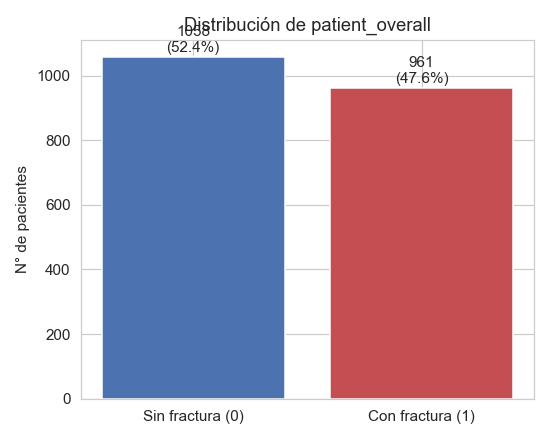
\includegraphics[width=.48\linewidth]{01_patient_overall.png}\hfill
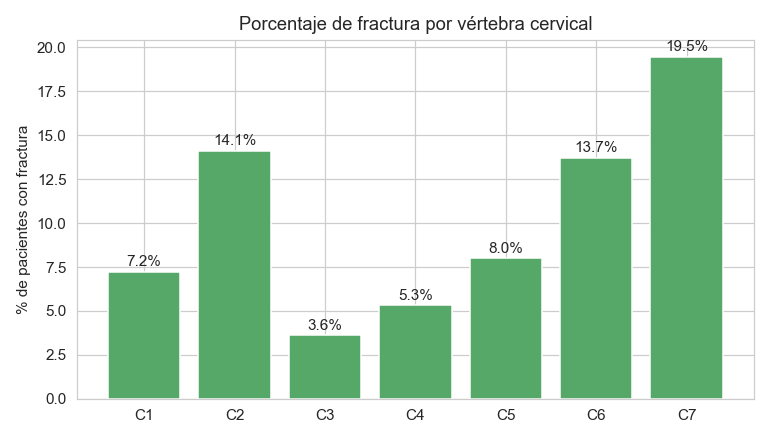
\includegraphics[width=.48\linewidth]{02_frac_por_vertebra.png}
\caption{An\'alisis exploratorio tabular (primera entrega): distribuci\'on de la variable objetivo \texttt{patient\_overall} y frecuencia de fractura por v\'ertebra.}
\end{figure}

\subsection{Limpieza y preprocesamiento}
En los CSV no hubo valores nulos ni filas duplicadas, \texttt{StudyInstanceUID} es \'unico y \texttt{patient\_overall} es consistente con la suma de C1--C7, por lo que no se aplicaron correcciones a las etiquetas. En las im\'agenes, la variabilidad de metadatos no se corrige en los archivos sino en el \emph{pipeline} (secci\'on~\ref{sec:eda-dicom}): HU calculadas con el \texttt{RescaleSlope}/\texttt{RescaleIntercept} de cada archivo, ordenamiento por posici\'on $z$ y redimensionado a $224\times224$.

\subsection{An\'alisis exploratorio de las im\'agenes DICOM}\label{sec:eda-dicom}
\paragraph{Fuente y tama\~no de muestra.} El an\'alisis usa la auditor\'ia del \emph{pipeline} (\cifFuente): \cifNEstudios{} estudios y \cifCortesLeidos{} cortes (los 48 centrales de cada estudio). El n\'umero de cortes por estudio es el total de archivos del estudio; el resto de metadatos proviene \'unicamente de esos 48 cortes. El notebook \texttt{notebooks/02\_eda\_imagenes.ipynb} y el script \texttt{scripts/eda\_metadatos\_dicom.py} permiten repetir el an\'alisis leyendo las cabeceras de \emph{todos} los cortes de una muestra estratificada (semilla 42) directamente en Kaggle.

\paragraph{Estad\'istica descriptiva.}
\begin{table}[H]\centering\small\tablaDesc
\caption{Estad\'istica descriptiva por estudio (\cifNEstudios{} estudios).}
\end{table}
El grosor de corte toma pocos valores discretos (mediana 0.625~mm, m\'aximo 1~mm, en l\'inea con el criterio de inclusi\'on del conjunto de datos de grosor $\le 1$~mm; \citealp{lin2023rsna}), mientras que el tama\~no de p\'ixel var\'ia entre 0.19 y 0.713~mm; el n\'umero de cortes cubre un rango de m\'as de un orden de magnitud. Tras redimensionar a $224\times224$, el tama\~no f\'isico del p\'ixel resultante var\'ia entre estudios, pues no se remuestrea de forma isotr\'opica.

\begin{figure}[H]\centering
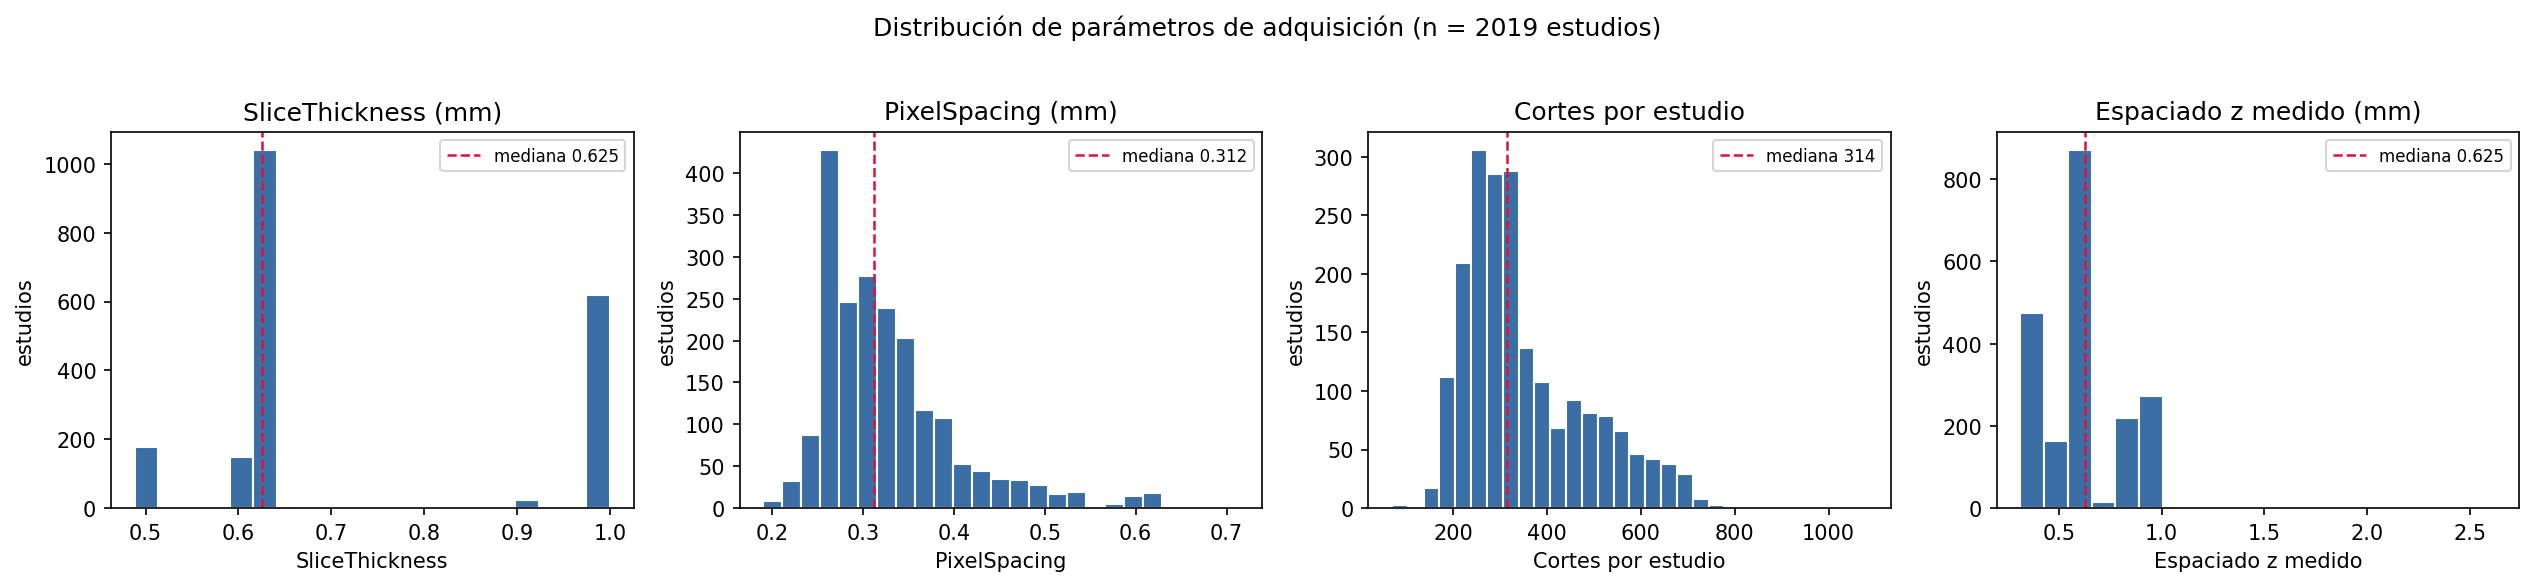
\includegraphics[width=\linewidth]{01_distribuciones_adquisicion.png}
\caption{Distribuciones de cortes por estudio, SliceThickness, PixelSpacing y espaciado $z$ medido.}
\end{figure}
\begin{figure}[H]\centering
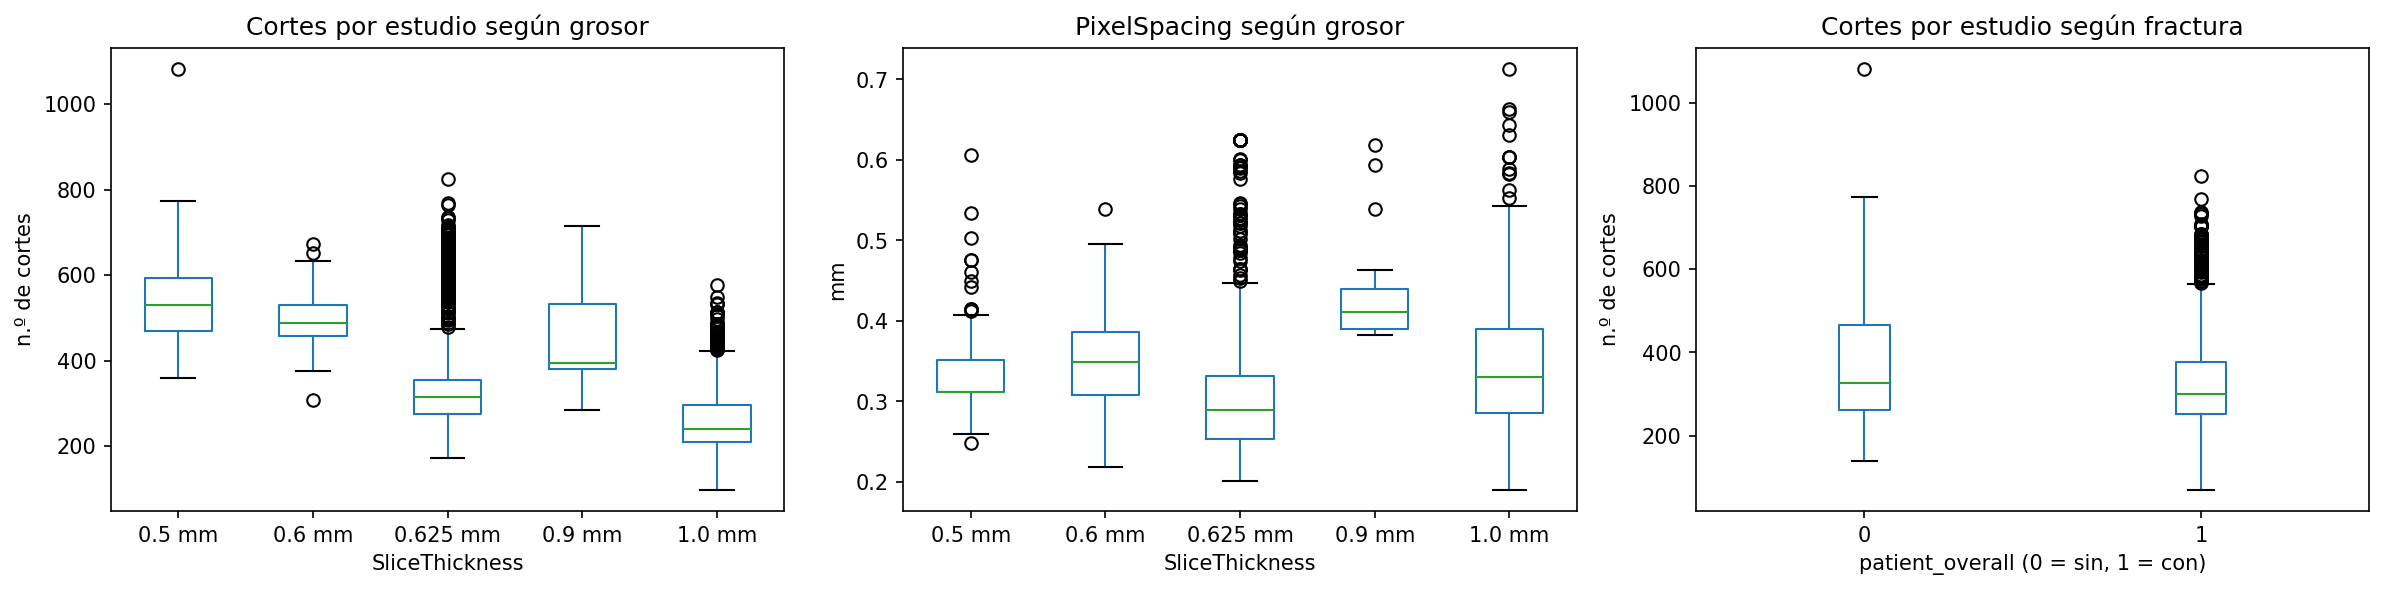
\includegraphics[width=\linewidth]{02_boxplots_comparacion.png}
\caption{Comparaci\'on de par\'ametros de adquisici\'on seg\'un \texttt{patient\_overall} (descriptiva; sin prueba de hip\'otesis).}
\end{figure}
\begin{figure}[H]\centering
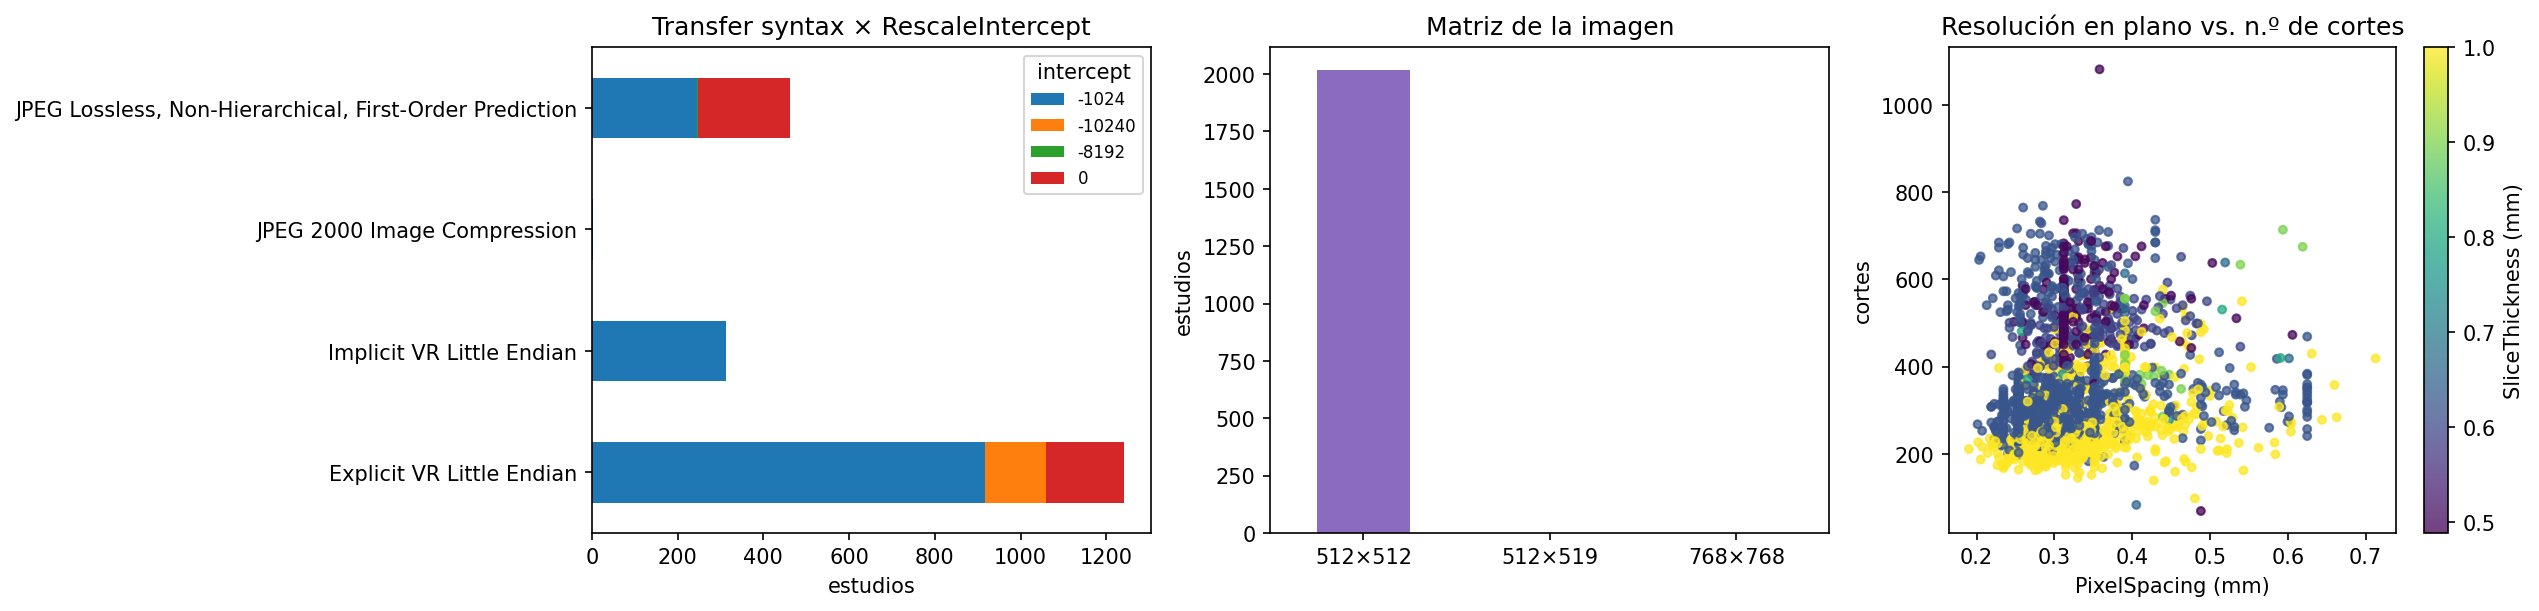
\includegraphics[width=\linewidth]{03_protocolos_y_resolucion.png}
\caption{Protocolos de reescalado, sintaxis de transferencia y resoluci\'on de matriz.}
\end{figure}

\paragraph{Valores at\'ipicos y metadatos inconsistentes.}
\begin{table}[H]\centering\small\tablaChecks
\caption{Comprobaciones de calidad sobre los metadatos. Los umbrales de at\'ipicos usan IQR$\times$1.5.}
\end{table}
Los hallazgos relevantes para el preprocesamiento son: (i) \cifNInterceptAtip{} estudios (\cifNInterceptAtipPct\,\%) con \texttt{RescaleIntercept} distinto de $-1024$ y $0$: 141 con intercept $-10240$ y \texttt{RescaleSlope} $=10$, y 3 con intercept $-8192$; (ii) \cifNNoQuinientos{} estudios que no son $512\times512$; (iii) ning\'un estudio con dimensiones, grosor o reescalado variables \emph{dentro} del estudio, ni fotometr\'ia distinta de MONOCHROME2; (iv) \cifNOutPixel{} estudios con \texttt{PixelSpacing} at\'ipico y \cifNOutCortes{} con n\'umero de cortes at\'ipico. Que las HU resultantes de los estudios con reescalado at\'ipico sean plausibles se comprueba con p\'ixeles reales y no con metadatos (v\'ease m\'as abajo).

\paragraph{Orden de los cortes y auditor\'ia del \emph{pipeline}.}
El sentido de $z$ respecto al n\'umero de instancia no es constante: \cifZDecr{} estudios son decrecientes, \cifZCrec{} crecientes y \cifZMixto{} mixto; \cifZNoMono{} estudio no es mon\'otono. Los estudios con espaciado $z$ irregular o no mon\'otono son \cifZAnomalos{} (identificados por los \'ultimos d\'igitos de su UID). Esto justifica ordenar por \texttt{ImagePositionPatient[2]} y no por n\'umero de instancia. El sentido creciente es m\'as frecuente en estudios positivos (\cifPosCrecPct\,\% frente a \cifNegCrecPct\,\% en negativos; $\chi^2$, $p=\cifChiP$); es una asociaci\'on descriptiva que podr\'ia reflejar diferencias de protocolo o instituci\'on, que los metadatos disponibles no permiten confirmar.
El preprocesamiento de los \cifNEstudios{} estudios termin\'o con \cifFallosPrep{} fallos; el tiempo por estudio fue de \cifTMedia{}~s en promedio (mediana \cifTMediana{}~s, m\'aximo \cifTMax{}~s) y los estudios comprimidos con JPEG Lossless tardaron aproximadamente el doble que los no comprimidos (mediana 4.07~s frente a 2.11~s con Explicit VR Little Endian).

\begin{figure}[H]\centering
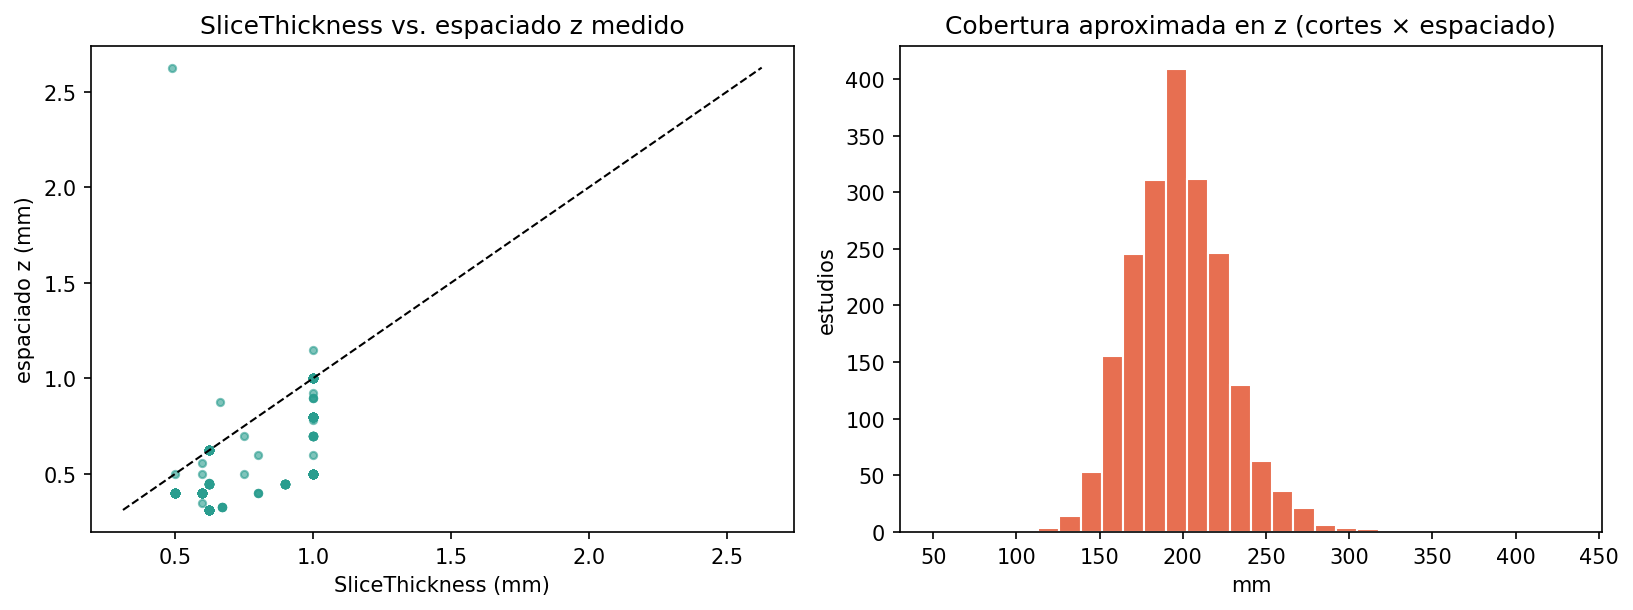
\includegraphics[width=\linewidth]{04_consistencia_z.png}
\caption{Consistencia del eje $z$ entre estudios.}
\end{figure}
\begin{figure}[H]\centering
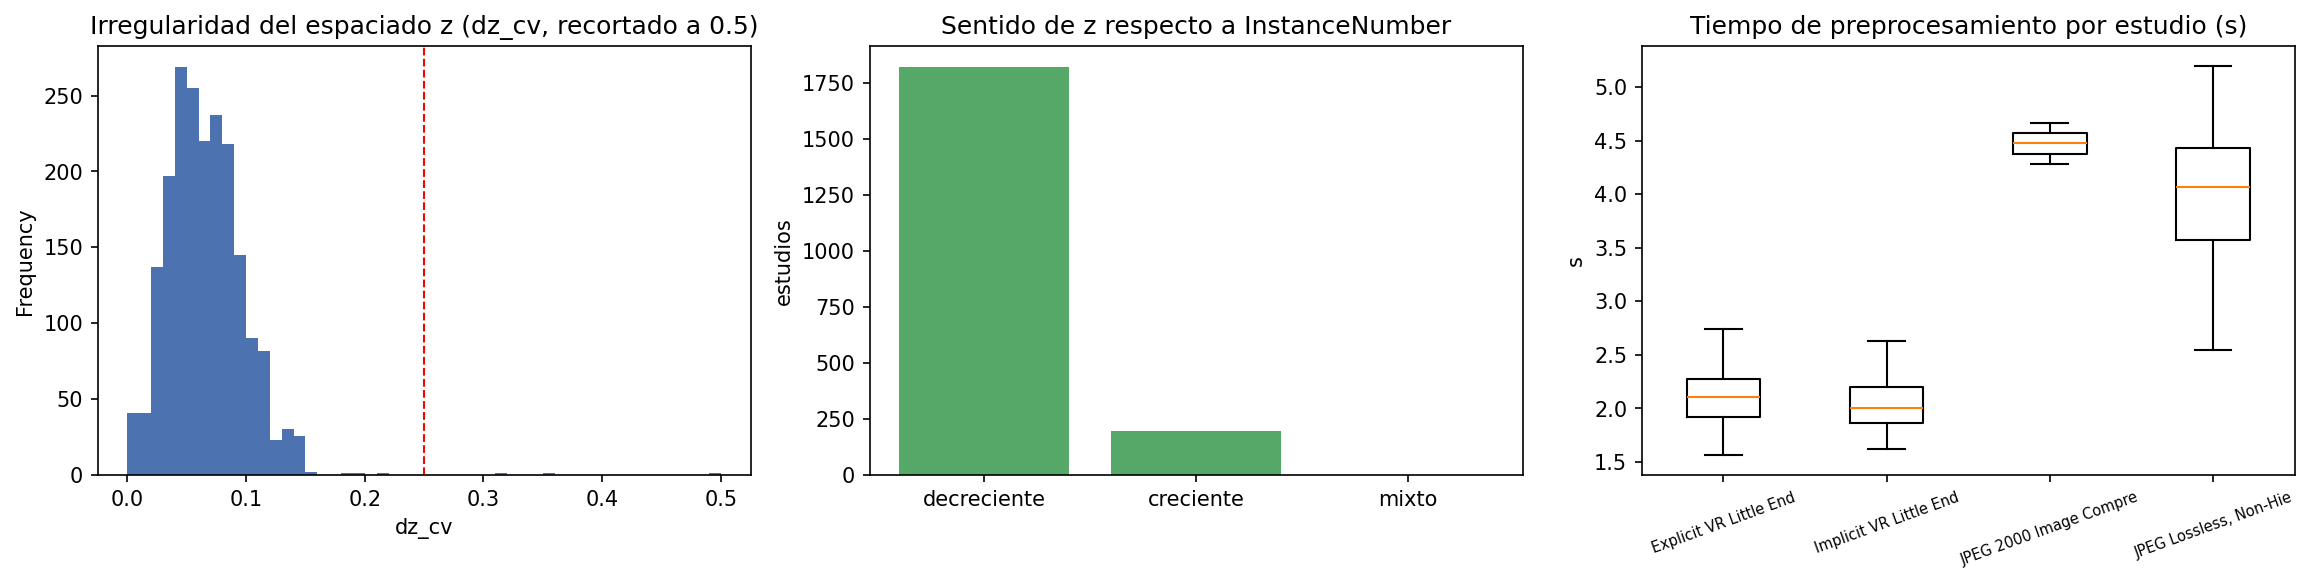
\includegraphics[width=\linewidth]{07_auditoria_pipeline.png}
\caption{Auditor\'ia del \emph{pipeline}: irregularidad del espaciado $z$, sentido de $z$ y tiempo de preprocesamiento por sintaxis de transferencia.}
\end{figure}

\paragraph{Ejemplos reales antes y despu\'es del preprocesamiento.}
Las figuras siguientes provienen del \emph{pipeline} de entrenamiento (\texttt{artifacts/v2/results/figures/}) y muestran el corte en HU crudo, el histograma con la ventana \'osea y el resultado final.
\begin{figure}[H]\centering
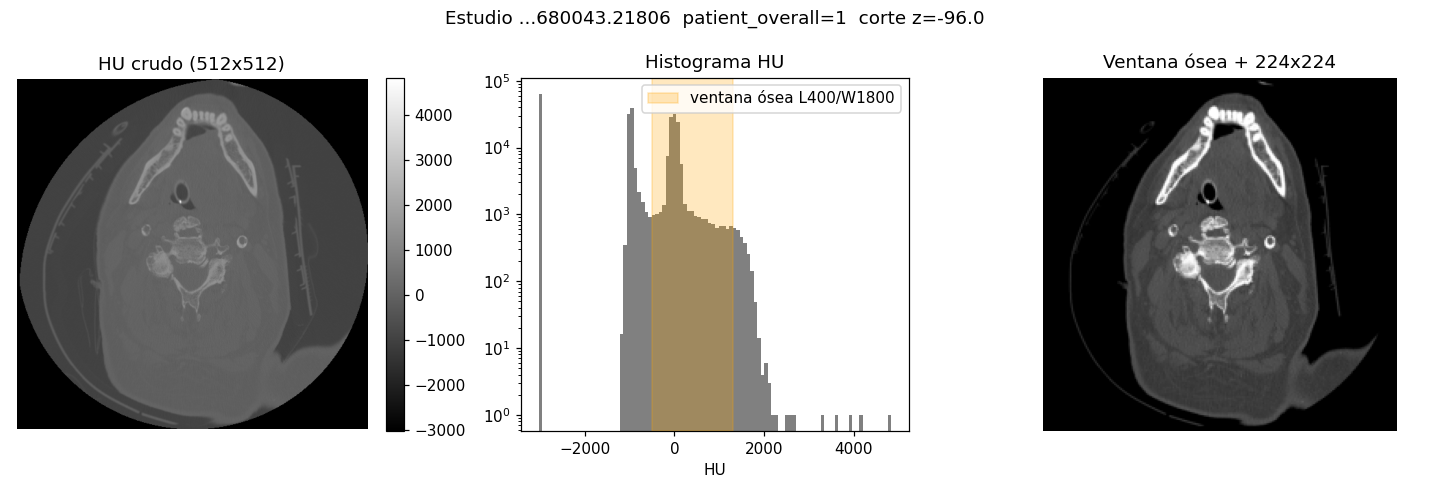
\includegraphics[width=\linewidth]{preproc_antes_despues_y1_21806.png}\\[3pt]
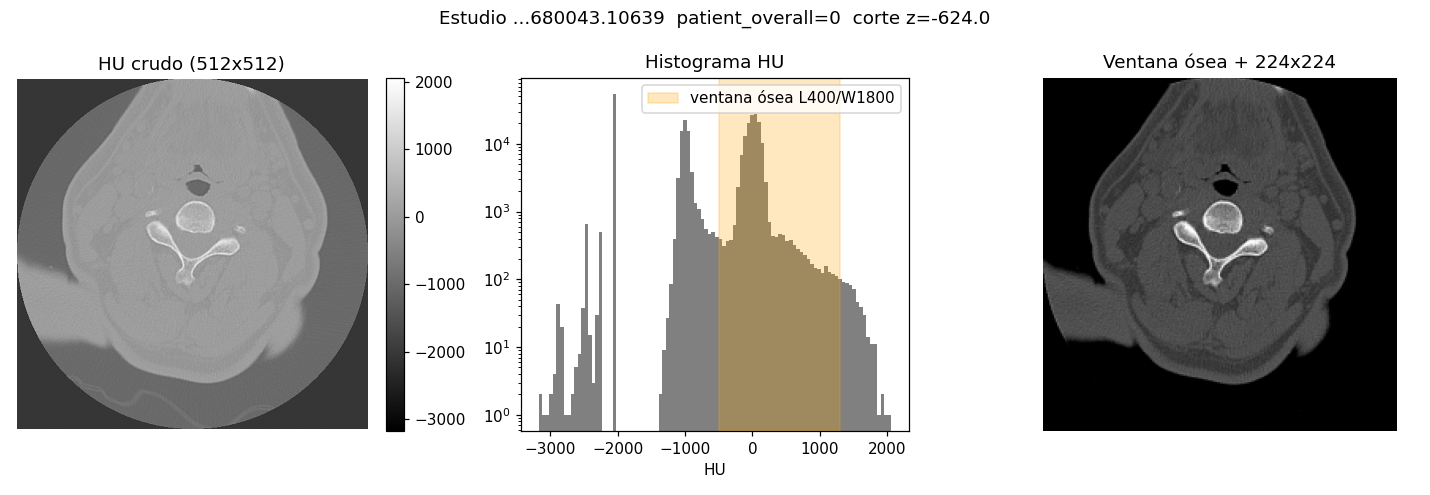
\includegraphics[width=\linewidth]{preproc_antes_despues_y0_10639.png}
\caption{Antes y despu\'es del preprocesamiento en un estudio positivo (arriba) y uno negativo (abajo).}
\end{figure}
\pendiente{Intensidades (HU) por grupo de reescalado y diferencias de adquisici\'on}{Histogramas de HU del corte central de una submuestra, con todos los estudios de reescalado at\'ipico y estudios aleatorios, y la comparaci\'on antes/despu\'es sobre ellos (secci\'on~5 del notebook 02).}{Ejecuci\'on de \texttt{notebooks/02\_eda\_imagenes.ipynb} en Kaggle con la competencia como entrada (produce \texttt{intensidades\_corte\_central.csv} y las figuras 05 y 06).}

\paragraph{Limitaciones del EDA de im\'agenes.}
\begin{itemize}[nosep]
\item Solo se dispone de las cabeceras de 48 cortes centrales por estudio; no se pueden detectar huecos en $z$ ni cabeceras at\'ipicas fuera de esos cortes.
\item El espaciado $z$ medido es la distancia entre dos cortes consecutivos \emph{muestreados}, no una mediana del estudio. Por ello la comparaci\'on grosor\,\,vs.\,\,espaciado $z$ (\cifNGrosorSpacing{} estudios, \cifNGrosorSpacingPct\,\%) no es concluyente y se excluye de la tabla de calidad hasta confirmarla con cabeceras completas.
\item Las comprobaciones sobre cabeceras no sustituyen una revisi\'on cl\'inica de la calidad de imagen ni miden artefactos (metal, movimiento).
\item La comparaci\'on por \texttt{patient\_overall} es descriptiva, sin control de confusores de protocolo.
\end{itemize}

\subsection{Ajuste de par\'ametros}
\pendiente{Ajuste de par\'ametros de cada algoritmo (responsable GPU)}{Qu\'e par\'ametros se ajustaron, c\'omo y con qu\'e efecto sobre el rendimiento.}{Texto de la responsable GPU; historiales en \texttt{artifacts/v2/results/history\_*.csv}.}

\subsection{Comparaci\'on de algoritmos}
\pendiente{Comparaci\'on de modelos y selecci\'on (P3)}{Tabla comparativa de m\'etricas, pruebas estad\'isticas pareadas, tiempos y figuras est\'aticas (ROC, matrices de confusi\'on, distribuci\'on de probabilidades) con interpretaci\'on y modelo seleccionado.}{An\'alisis y redacci\'on de P3 (Hansel); datos en \texttt{artifacts/v2/results/} y \texttt{notebooks/03\_evaluacion.ipynb} (rama \texttt{main}).}

\subsection{Aplicaci\'on desarrollada}
\pendiente{Aplicaci\'on Streamlit (P1)}{Descripci\'on de la aplicaci\'on, capturas de pantalla y justificaci\'on de las tecnolog\'ias elegidas.}{Capturas y documentaci\'on de P1 (Cabrera): \texttt{docs/app/capturas/} y \texttt{docs/app/SECCION\_INFORME\_APP.md} (rama \texttt{main}).}

\section{Conclusiones}
\pendiente{Conclusiones (P3)}{C\'omo se cumplieron cada uno de los objetivos de la secci\'on~2 y discusi\'on de la efectividad de los algoritmos. Se redactan solo a partir de los resultados reales de la comparaci\'on.}{Redacci\'on de P3 (Hansel) a partir de \texttt{artifacts/v2/results/}.}

\subsection*{Conclusiones del EDA de im\'agenes (P2)}
La heterogeneidad de los metadatos DICOM es real y medible: reescalado at\'ipico en \cifNInterceptAtipPct\,\% de los estudios, tama\~nos de p\'ixel entre 0.19 y 0.713~mm, sentido de $z$ variable y compresi\'on distinta entre estudios. Las decisiones del \emph{pipeline} (HU por archivo, orden por $z$, ventana \'osea) responden a esa heterogeneidad. Quedan abiertas dos verificaciones que requieren p\'ixeles: la plausibilidad de las HU en los estudios con reescalado at\'ipico y el an\'alisis de intensidades por grupo de adquisici\'on (ver el recuadro de pendientes en la secci\'on~\ref{sec:eda-dicom}).

\subsection*{Limitaciones generales}
Una sola partici\'on y una sola semilla; 48 posiciones por estudio de cientos de cortes (la fractura puede no estar muestreada); clasificador global que no localiza la fractura; sin remuestreo isotr\'opico; sin validaci\'on cl\'inica ni externa, por lo que las m\'etricas no son comparables con las de la competencia.


\bibliographystyle{apalike}
\bibliography{referencias}

\appendix
\section{Estado de integraci\'on del informe (uso interno; eliminar antes de entregar)}
\begin{table}[H]\centering\small
\begin{tabular}{p{4.2cm}p{3.2cm}p{6.5cm}}\toprule
Secci\'on & Responsable & Estado \\\midrule
Introducci\'on, marco te\'orico (TC, DL, evaluaci\'on) & P2 (integraci\'on) & Redactado a partir del borrador del equipo \\
Anatom\'ia y fracturas (marco te\'orico m\'edico) & Revisi\'on bibliogr\'afica & Pendiente de integrar desde el .docx \\
Datos, particiones, preprocesamiento & P2 / GPU & Redactado con cifras v2 (verificar con GPU) \\
Metodolog\'ia de entrenamiento y ajuste & Responsable GPU & Pendiente \\
EDA de im\'agenes (metadatos, orden $z$, tiempos) & P2 & Con cifras reales de la auditor\'ia \\
EDA de im\'agenes (intensidades HU, antes/despu\'es propios) & P2 & Pendiente de ejecuci\'on en Kaggle \\
Comparaci\'on de modelos y conclusiones & P3 & Pendiente \\
Aplicaci\'on y capturas & P1 & Completo (inferencia real validada en 2 estudios de prueba) \\
Resumen & Todos & Pendiente (al cierre) \\\bottomrule
\end{tabular}
\caption{Matriz de integraci\'on. Los recuadros amarillos del texto son los espacios reservados.}
\end{table}

\end{document}
